\hypertarget{framegen_8c}{
\section{framegen.c File Reference}
\label{framegen_8c}\index{framegen.c@{framegen.c}}
}
{\tt \#include $<$stdio.h$>$}\par
{\tt \#include $<$stdlib.h$>$}\par
{\tt \#include $<$string.h$>$}\par
{\tt \#include $<$unistd.h$>$}\par
{\tt \#include \char`\"{}dcsc\-Msg\-Buffer\-Interface.h\char`\"{}}\par
{\tt \#include \char`\"{}framegen.h\char`\"{}}\par


Include dependency graph for framegen.c:\begin{figure}[H]
\begin{center}
\leavevmode
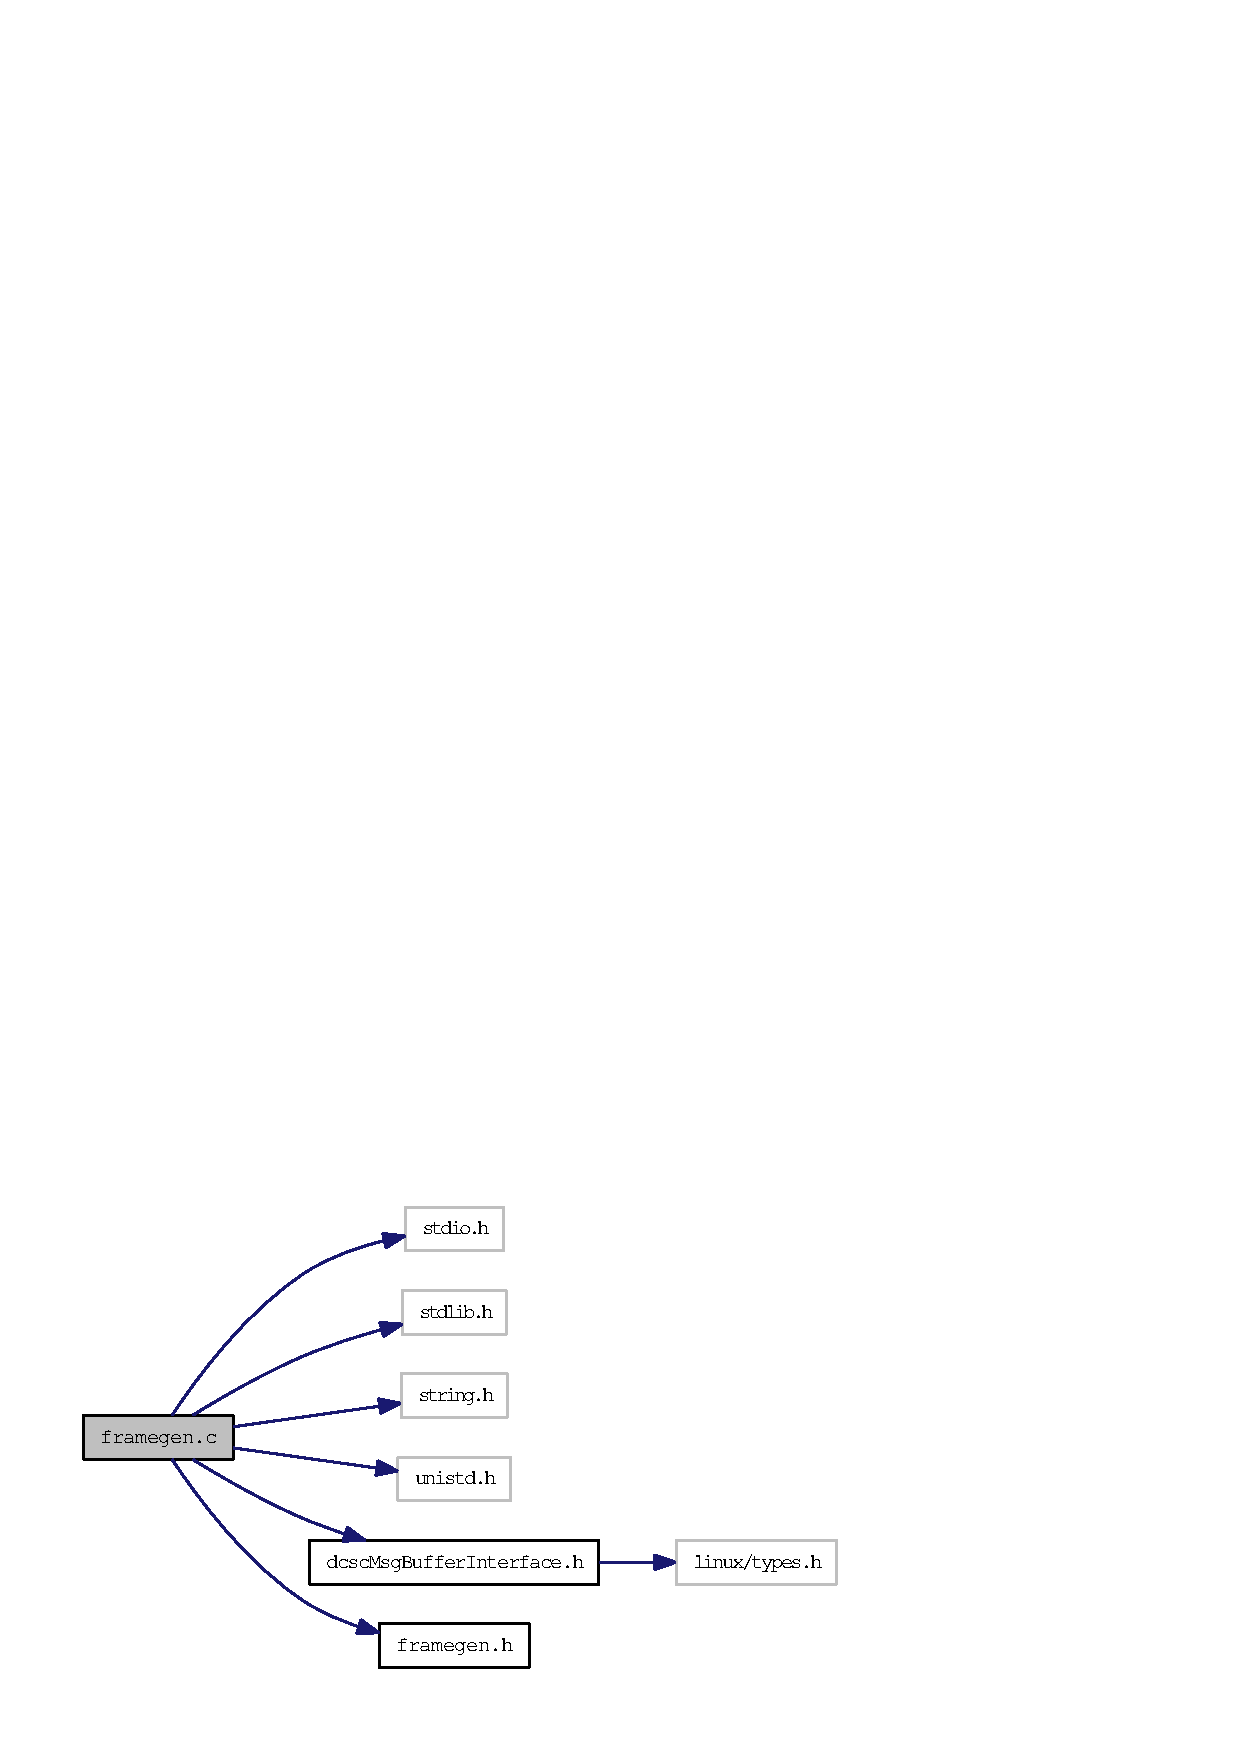
\includegraphics[width=203pt]{framegen_8c__incl}
\end{center}
\end{figure}
\subsection*{Functions}
\begin{CompactItemize}
\item 
int \hyperlink{framegen_8c_64470613eeeb13398e90523259a10d8b}{commit} ()
\begin{CompactList}\small\item\em executes a previously written command \item\end{CompactList}\item 
int \hyperlink{framegen_8c_3c04138a5bfe5d72780bb7e82a18e627}{main} (int argc, char $\ast$$\ast$argv)
\end{CompactItemize}


\subsection{Function Documentation}
\hypertarget{framegen_8c_64470613eeeb13398e90523259a10d8b}{
\index{framegen.c@{framegen.c}!commit@{commit}}
\index{commit@{commit}!framegen.c@{framegen.c}}
\subsubsection[commit]{\setlength{\rightskip}{0pt plus 5cm}int commit ()}}
\label{framegen_8c_64470613eeeb13398e90523259a10d8b}


executes a previously written command 

\begin{Desc}
\item[Returns:]the errorcode \end{Desc}


Definition at line 31 of file framegen.c.

References rcu\-Single\-Write().

Referenced by main().

Here is the call graph for this function:\begin{figure}[H]
\begin{center}
\leavevmode
\includegraphics[width=394pt]{framegen_8c_64470613eeeb13398e90523259a10d8b_cgraph}
\end{center}
\end{figure}
\hypertarget{framegen_8c_3c04138a5bfe5d72780bb7e82a18e627}{
\index{framegen.c@{framegen.c}!main@{main}}
\index{main@{main}!framegen.c@{framegen.c}}
\subsubsection[main]{\setlength{\rightskip}{0pt plus 5cm}int main (int {\em argc}, char $\ast$$\ast$ {\em argv})}}
\label{framegen_8c_3c04138a5bfe5d72780bb7e82a18e627}




Definition at line 43 of file framegen.c.

References commit(), EXIT\_\-FAILURE, get\-Frame\-Address\-From\-Line(), get\-Hex\-Value\-From\-Line(), init\-Rcu\-Access(), rcu\-Multiple\-Read(), rcu\-Single\-Write(), and release\-Rcu\-Access().

Here is the call graph for this function:\begin{figure}[H]
\begin{center}
\leavevmode
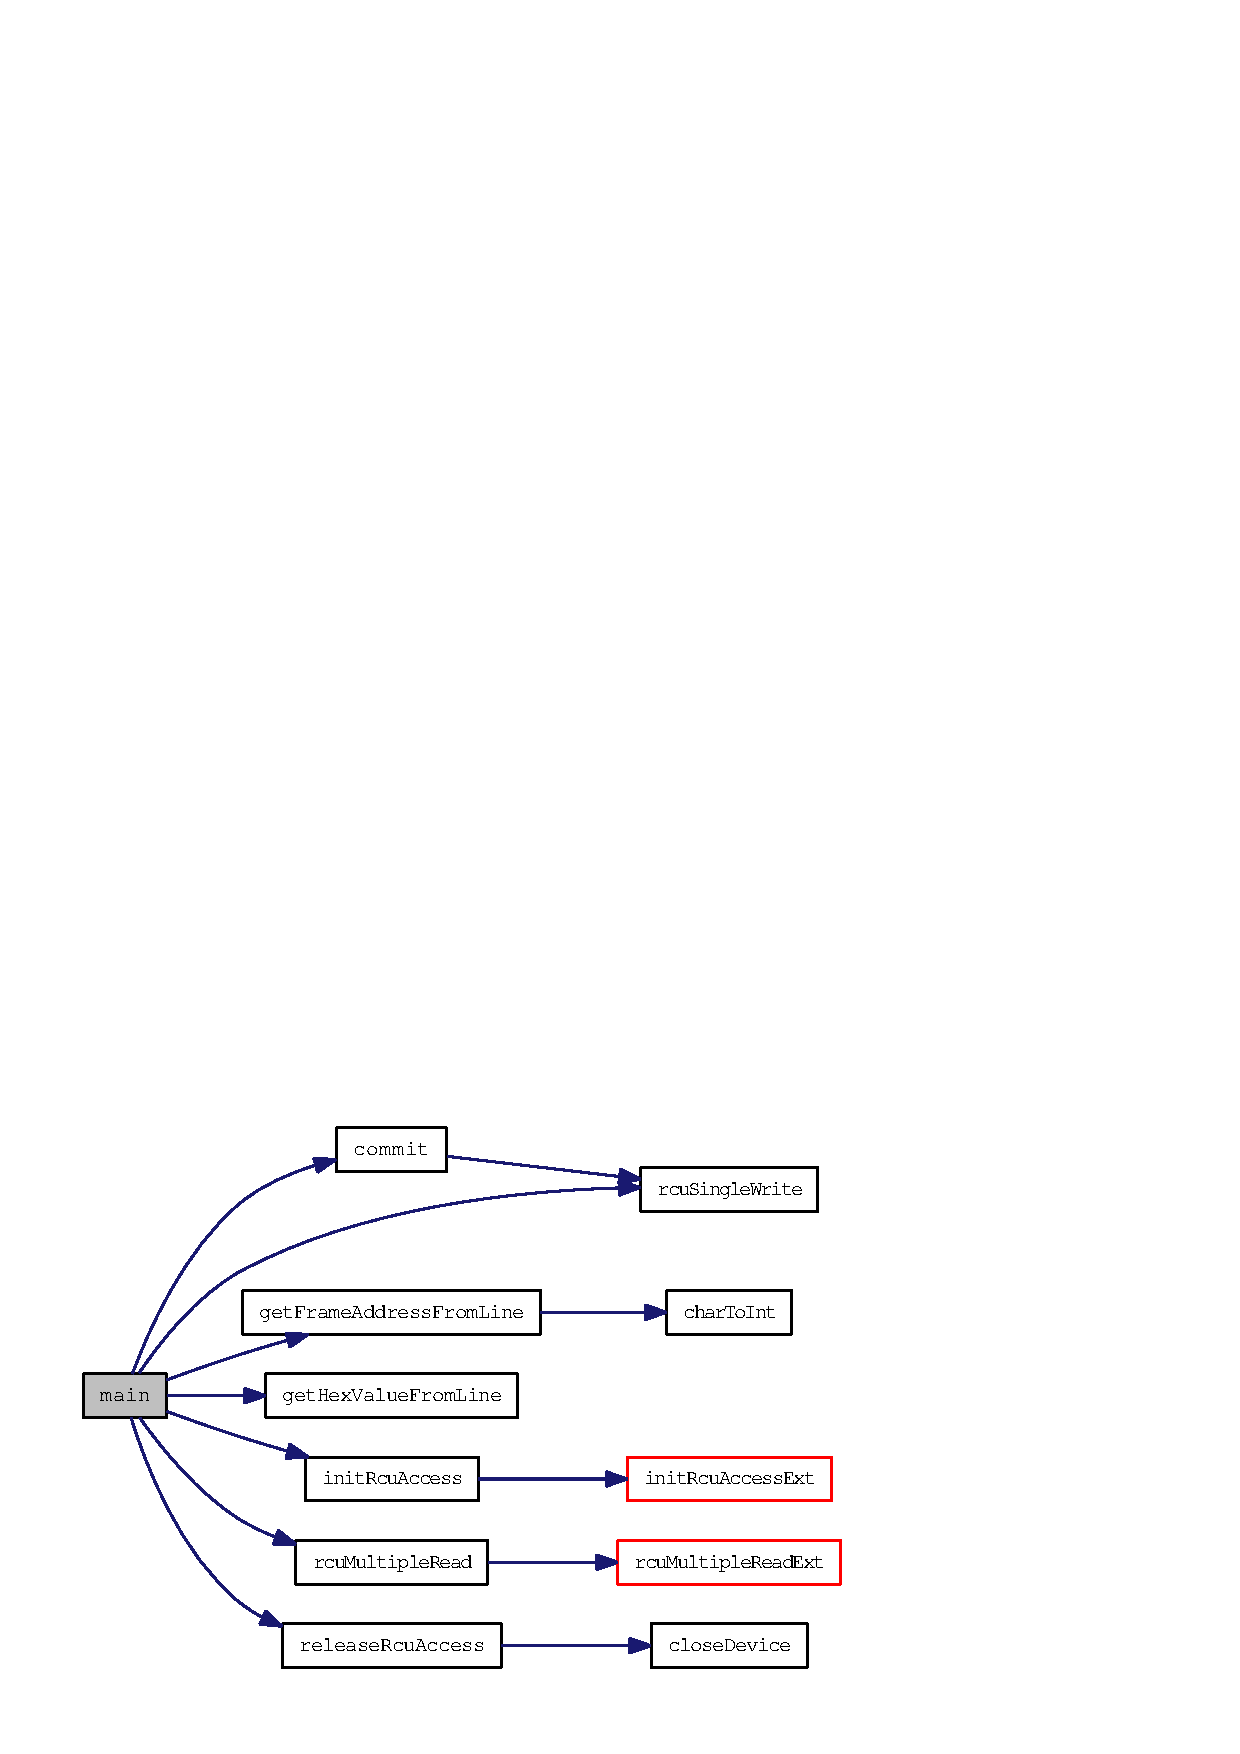
\includegraphics[width=204pt]{framegen_8c_3c04138a5bfe5d72780bb7e82a18e627_cgraph}
\end{center}
\end{figure}
